\subsection{Map Editor}\label{sprint2:map_editor}
The map editor has been developed due to \cref{sprint2:tab1:req11} and \cref{sprint2:tab1:req12} in \cref{sprint2:requirement_table_1}.
The map editor makes it possible for the user to make a map that fits to the citizen's needs.
A screenshot can be seen on \cref{fig:sprint2:map_editor}, where there are added two obstacles.
The map editor is a screen of the game with only garages.
Users are able to add an obstacle by touching the screen - and the obstacle will be placed there.
Users can remove an obstacle by touching it.

\begin{figure}[h]
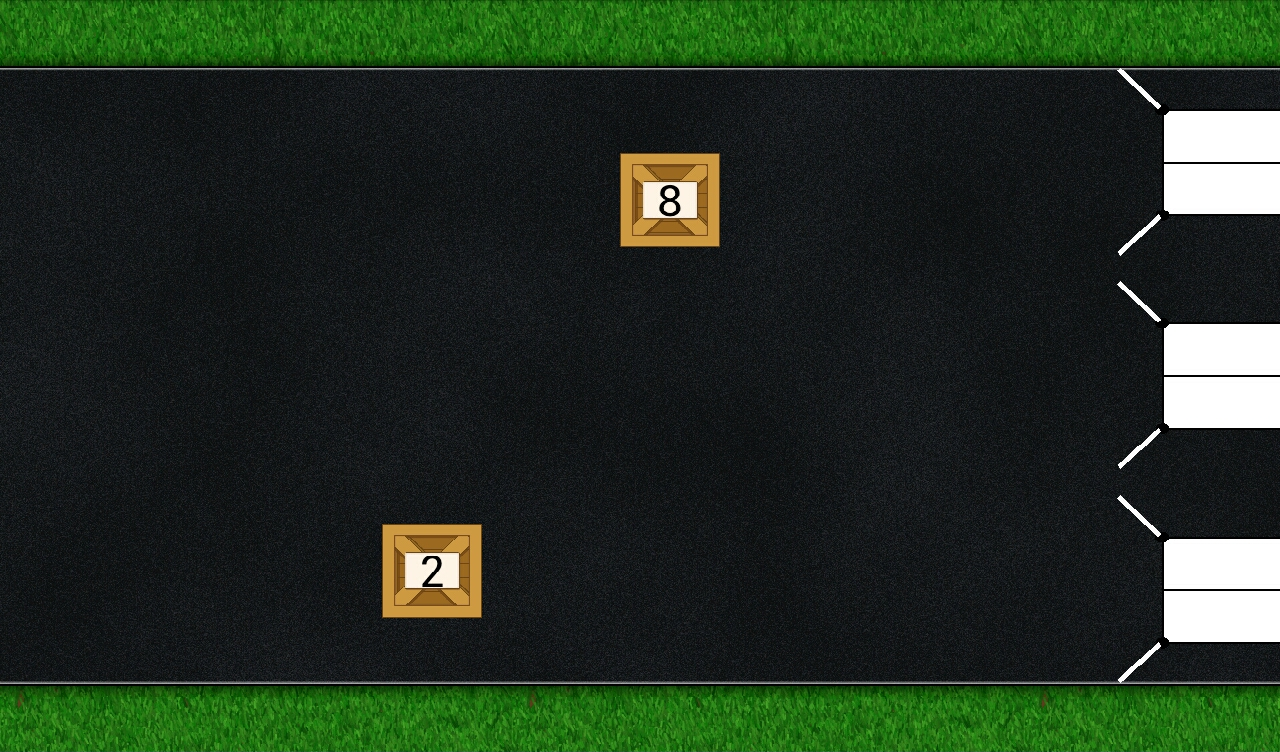
\includegraphics[width=\linewidth]{sprint2/map_editor}
\caption{The map editor, which makes it possible to customize the obstacle placement.}
\label{fig:sprint2:map_editor}
\end{figure}
 
